\chapter{Metode}
\textit{I dette kapitel beskrives formålet med udviklingen af beslutningsstøttesystem til risikovurdering af lægemidler, hvordan data er indsamlet samt hvilken proces der er gennemgået i forhold til udvikling for algoritme til risikovurdering som beslutningsstøtte.}

\section{Formål}
På nuværende tidspunkt vurderes kompleksiteten af implementering af lægemiddelskift af ATC-ansvarlige ud fra tidligere erfaringer og viden indsamlet via bl.a. pro.medicin. Flere faktorer vægtes ved vurderingen, hvilket gør denne proces meget personafhængig og stiller visse krav til den ATC-ansvarliges viden og erfaring inden for området. Vurderingen der foretager har betydning for implementeringen af lægemiddelskiftet i klinikken og det er derfor vigtigt at den rette vurdering foretages i forhold til at undgå medicineringsfejl som f.eks. forveksling af navn på lægemidlet grundet ændringer af navn ved lægemiddelskift.
For at imødekomme disse problemstillinger ønskes det at udvikle et beslutningsstøttesystem til den ATC-ansvarlige som foretager risikovurderingen af lægemiddelskift med henblik på at synliggøre de ændringer som sker ved et eventuelt lægemiddelskift, hvormed den ATC-ansvarlige har et bedre beslutningsgrundlag.

\section{Dataindsamling}
Data er indsamlet af Amgros og Sygehusapoteket Region Nordjylland (SRN) og omhandler lægemiddelskift i år 2018. Data fra Amgros omhandler oplysninger om lægemiddelskift i år 2017 og 2018. Yderligere har Amgros udarbejdet et dokument over risikolægemidler. Risikolægemidler er lægemidler som er særligt risikofyldte hvis disse ender i restordre, da erstatninger er svære at finde samt risikoen for fejl øges ved erstatning. Data fra SRN omhandler de udbud af lægemidler Amgros foretog inden et eventuelt kontraktskift for år 2018. 
%Udover dette har SRN ligeledes indsamlet de problemstillinger der har været vedrørende Amgrosskift siden år 2012.  


\section{Udviklingsproces}
Udviklingen af et beslutningsstøttesystem bygger på forskellige processer herunder valg af features, præprocessering, design, implementering og test. Udviklingstrin fremgår af Figur \ref{fig:metode}.

\begin{figure}[H]\centering	\includegraphics[width=1\textwidth]{billeder/udviklingstrin.png} 
	\caption{Udviklingstrin for beslutningsstøttesystem}
	\label{fig:metode}  
\end{figure}
\vspace{-0.5cm}
%Første trin omhandler identificering af problemer som systemet skal løse, herunder data som systemet skal arbejde på og tilgængelige ressourcer~\citep{Ligeza2006}. Det andet trin er omhandler identificering af nøglekoncepter samt relationer mellem disse som f.eks. typer af data, informationsstrøm og underliggende stukturer. Tredje trin involverer forståelse, beskrivelse og formalisering af problemet og hvordan løsninger findes. Denne proces bør omfatte verificering af systemet. Det fjerde trin har til formål at implementere den formaliseret viden i et program. Det sidste trin omfatter test ved validering af regler og implementeringen.~\citep{Ligeza2006}


\chapter{Systemanalyse}
\section{Valg af features}
Features er udvalgt på baggrund af retningslinjer for den ATC-ansvarlige, som fremgår af Appendiks~\ref{cha:AppD}, og litteratur som beskriver ændringer i forskellige faktorer som har ledt til medicineringsfejl i klinikken som følge af lægemiddelskift. Derudover er information omkring risikolægemidler og komplekse ATC-koder anvendt som er indsamlet af Amgros eller er dokumenteret i forbindelse med Amgrosudbud af SRN.
Features og begrundelse for valg af features fremgår af Tabel \ref{table:features}.

\begin{table}[H]
\caption{Valg af features}
\label{table:features}
\vspace{0.5cm}
\begin{tabular}{p{3.5cm} | p{11cm}}
{\cellcolor[HTML]{C0C0C0}\textbf{Feature}} & {\cellcolor[HTML]{C0C0C0}\textbf{Begrundelse}} \vspace{2mm} \\ \hline \vspace{0.1mm}
\textbf{Navn} & \vspace{0.1mm} Forveksling ved ændringer i navn på lægemidler er en af de hyppigste årsager til medicineringsfejl jævnfør afsnit \ref{sec:ProblemLaeg} [X]. Forvirring over ikke at kunne finde lægemidlet fordi navnet har ændret sig \\  \hline \vspace{0.1mm}
\textbf{Lignende navne} & \vspace{0.1mm}  Forveksling ved ændringer i navn på lægemidler er en af de hyppigste årsager til medicineringsfejl jævnfør afsnit \ref{sec:ProblemLaeg}. [X] Disse forekommer grundet allerede eksisterende lægemiddel jævnfør afsnit \ref{sec:ProblemLaeg}. [X]. \\  \hline \vspace{0.1mm}
\textbf{Dispenseringsform} & \vspace{0.1mm} FIND BEGRUNDELSE FOR DETTE  \\ \hline \vspace{0.1mm}
\textbf{Styrke} & \vspace{0.1mm} Forkert dosis er dokumenteret se kilde 18,19,20 og 21  \\ \hline \vspace{0.1mm}
\textbf{Risikolægemidler} & \vspace{0.1mm} Disse lægemidler kan være problematiske, hvis de ender i restordre, altså at lægemidlet ikke kan leveres og det derfor er nødvendigt at finde et erstatningslægemiddel. Disse lægemidler bør være på lager, da det er svært at finde erstatninger for disse samt risikoen for fejl øges ved erstatning. [FIND KILDE, eller indsæt i appendiks]  \\ \hline \vspace{0.1mm}
\textbf{ATC-koder} & \vspace{0.1mm} Der er nogle ATC-koder som er mere komplekse end andre. Dette er f.eks. på områder som indgår i produktionen på Sygehusapoteket Region Nordjylland og væsker, hvor en ændring i leverandør typisk vil forårsage ændringer af device, hvilket kan skabe problemer i klinikken. [KILDE] \\ \hline \vspace{0.1mm}
\textbf{Medicinråd} & \vspace{0.1mm} Nogle lægemidler omhandler medicinrådets behandlingsvejledninger. Disse lægemidler omfatter enkelte hospitalsafdelinger og kræver et tæt samarbejde med disse. Det ønskes ligeledes at lægemidlet implementeres hurtigt, da det er muligt at opnå store besparelser. [KILDE + APPENDIKS]\\ \hline \vspace{0.1mm}
\textbf{Pris} & \vspace{0.1mm} Pris er vigtigt i forhold til at opnå besparelser. Det skal ligeledes vægtes om det kan betale sig at skifte et lægemiddel med mindre besparelse, da udskiftningen kan få store betydninger for klinikken i forhold til arbejdsgangen og i værste tilfælde medføre patientsikkerhedsmæssige konsekvenser. [KILDE, AMGROS] \textit{Det er endnu ikke besluttet, hvordan denne faktor skal indgå i algoritmen.} \\ \hline
\end{tabular}
\end{table}



\section{Præprocessering}
Data er manuelt indskrevet og indeholder tekst og er derfor ikke sammenligneligt, hvorfor data er præprocesseret før anvendelsen. Da det er forskelligt om data er skrevet med majuskel eller minuskel er det valgt at ændre alt data til minuskel. Derudover er der i nogle tilfælde anvendt forkortelser og andre gange er ordet skrevet helt ud, hvorfor det er valgt at fjerne forkortelser og udskrive ordene med henblik på at gøre data generaliserbar. 

Derudover er der lavet antagelse for navn og dispenseringformer for lægemidler. For lægemidler med samme præfiks er der ikke foretaget en navneændring, hvorfor det er valgt at fjerne suffikser fra lægemidlernes navne. Dog kan suffikser have en betydning for ændringer i dispenseringsform og styrke, men det antages at disse ændringer vil gøre sig gældende i ændringer i dispenseringsform og styrke. Ligledes antages det for dispenseringsformer som tabletter at disse er ens hvis dispenseringsform er en af følgende; filmovertrukne, overtrukne eller  tabelletter.





\section{Design}
** Tænker at dette afsnit skal være et flowdiagram over der forskellige processer ala det billede jeg har sat ind ***


\begin{figure}[H]\centering	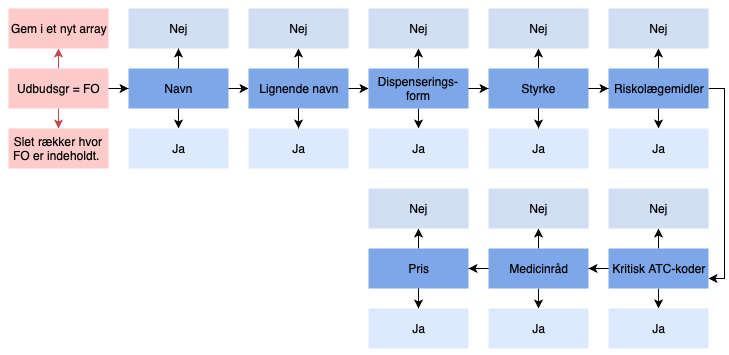
\includegraphics[width=1\textwidth]{billeder/algoritme.png} 
	\caption{Flowchart af algoritme}
	\label{fig:metode}  
\end{figure}
\vspace{-0.5cm}


\chapter{Implementering}
Netbeans - apache poi

** pseudo code som if-then sætninger **


\section{Test}
Tænker at teste noget i forhold til falsk/positive. Hvor mange gang gør algoritmen det den skal?

